%    Template for seminar reports
% Seminar Current Topics in Computer Vision and Machine Learning
% Summer Semester 2015
% Computer Vision Group, Visual Computing Institute, RWTH Aachen

\documentclass[twoside,a4paper,article]{combine}


% =========================================================================
\usepackage[utf8]{inputenc}
\usepackage[ngerman]{babel}
\usepackage{a4}
\usepackage{fancyhdr}   
%\usepackage{german}    % Uncomment this iff you're writing the report in German
\usepackage{makeidx}
\usepackage{color}
\usepackage{t1enc}		% german letters in the "\hyphenation" - command
\usepackage{latexsym}	% math symbols
\usepackage{amssymb}    % AMS symbol fonts for LaTeX.

\usepackage{graphicx}
\usepackage{pslatex}
\usepackage{ifthen}

\usepackage[T1]{fontenc}
\usepackage{pslatex}

\usepackage{psfrag}
\usepackage{subfigure}
\usepackage{url}

% =========================================================================

\setlength{\oddsidemargin}{3.6pt}
\setlength{\evensidemargin}{22.6pt}
\setlength{\textwidth}{426.8pt}
\setlength{\textheight}{654.4pt}
\setlength{\headsep}{18pt}
\setlength{\headheight}{15pt}
\setlength{\topmargin}{-41.7pt}
\setlength{\topskip}{10pt}
\setlength{\footskip}{42pt}

\setlength{\parindent}{0pt}

% =========================================================================

\graphicspath{
	{img/}
}

%%%
% We want also subsubsections to be enumerated
%%%
\setcounter{secnumdepth}{3}
\setcounter{tocdepth}{3}

\makeglossary
%\makeindex

% =========================================================================
\begin{document}

% Template for seminar reports
% Seminar Current Topics in Computer Vision and Machine Learning

\begin{titlepage}


\begin{center}
\ 
\vspace{3.5cm}


\textsf
{
Fakultät für Mathematik, Informatik und Naturwissenschaften\\
Lehr- und Forschungsgebiet Informatik VIII\\
Computer Vision\\
Prof. Dr. Bastian Leibe
}

\rule{\linewidth}{1pt}

\vspace{1.75cm}
\LARGE
\textbf{Seminar Report}

\vspace{1.7cm}
\huge
Combining 3D Shape, Color, and Motion for Robust Anytime Tracking

\vspace{3.0cm}
\Large
Frederik Zwilling\\
\large
Matriculation Number: 304314

\vspace{0.5cm}
June 2015

\vspace{1.05cm}
\rule{\linewidth}{1pt}

\vspace{0.5cm}
\textsf{\textbf{
\normalsize
\begin{tabular}{ll}
Advisor:  & Aljoša Ošep\\
\end{tabular}
}}
\end{center}

\end{titlepage}


\begin{abstract}
  \textcolor{red}{Abstract}
\end{abstract}

\tableofcontents
\newpage
% =========================================================================

\section{Introduction}


\subsection{Motivation}
Robotic applications are about to change many domains from the ground
up. Especially autonomous systems could take over dangerous,
exhausting and unpopular tasks and allow humans to do more satisfying
tasks instead. Additionally, autonomous systems can be more efficient
and scalable than solving the tasks by hand. Some progressive domains
with autonomous robots are flying drones, which can map
areas~\cite{auto-drones} or deliver
packages~\cite{auto-delivery-drones}, autonomous cars, which take care
of driving~\cite{auto-cars}, logistic robots, which store and grab
goods in warehouses~\cite{kiva}, and domestic service robots, which
can support old people and clean at home~\cite{athome}. All these
domains have in common that the robots have to track objects in their
environment, mostly for avoiding collisions, in the case of domestic
service robot also to follow people for example. Often the reliability
and precision of the tracking are limiting factors. An autonomous car,
for example, can only drive fast if it is absolutely sure that it
tracks all objects in the sorounding correctly and none of these
objects could cause a collision.  This report mainly focuses on the
domain of autonomous cars. Here, the autonomous system takes care of
the time consuming driving task on the one hand and could help to
reduce the amount of traffic deaths ($25,938$ in $2013$ in the
EU~\cite{traffic-deaths}) on the other hand. In this domain it is
especially important to estimate the speed of various nearby objects
robustly and in real time. Figure~\ref{fig:objects} shows the three
main classes of objects that have to be tracked, cars, bycicles, and
pedestrians, in challenging situations. The method proposed in this
report solves this task and performs better than previous approaches
in the car domain.
\begin{figure}
  \label{fig:objects}
  \subfigure[Cars on a highway]{%
    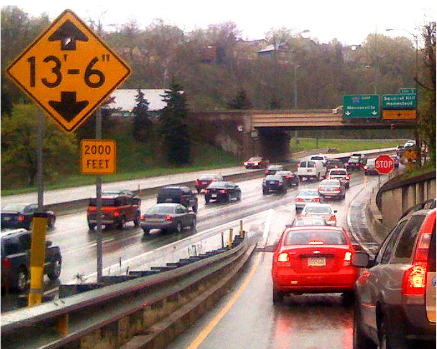
\includegraphics[height=.3\linewidth]{highway}
  }
  \subfigure[A cyclist]{%
    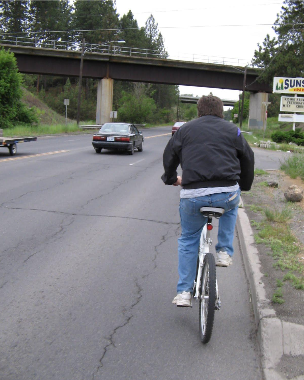
\includegraphics[height=.3\linewidth]{bicycle}
  }
  \subfigure[A pedestrian]{%
    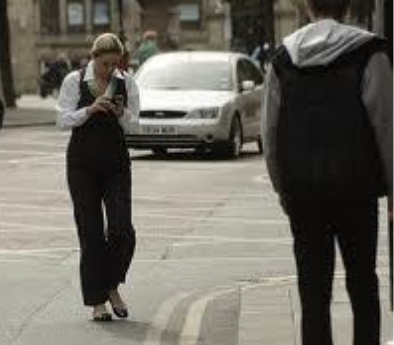
\includegraphics[height=.3\linewidth]{pedestrian}
  }
  
  \caption{Various objects that have to be tracked in challenging
    situations~\cite{held-website}}
\end{figure}


\subsection{Tracking}
\subsection{Velocity and Pose Estimation}
% +++++++++++++++++++++++++
\section{Related Work}
\subsection{Trajectory Classification}
\subsection{Grid-Based Methods}
\subsection{Alternative Sensors}

% +++++++++++++++++++++++++
\section{Method}
\subsection{Probabilistic Model}
\subsection{Annealed Dynamic Histograms}
\subsection{Adding Color}

% +++++++++++++++++++++++++
\section{Evaluation}
\subsection{Relative Reference Frame}
\subsection{Model Crispness}

% +++++++++++++++++++++++++
\section{Conclusion}


% =========================================================================
\bibliographystyle{alpha}
\bibliography{seminar_report}

% =========================================================================

\end{document}
